\newpage
\subsection{Umkehr-Funktionen}

\hfill \break
\begin{itemize}
    \item Grapisch wird die Umkehrfunktionen durch das Spiegeln an der 1.Mediane ermittelt
    \item Rechnerisch wird die Umkehrfunktionen durch das Vertauschen von x und y ermittelt. zb.
          $y=10^x \rightarrow x=10^y \rightarrow y=Lg(x)$
\end{itemize}

\hfill \break
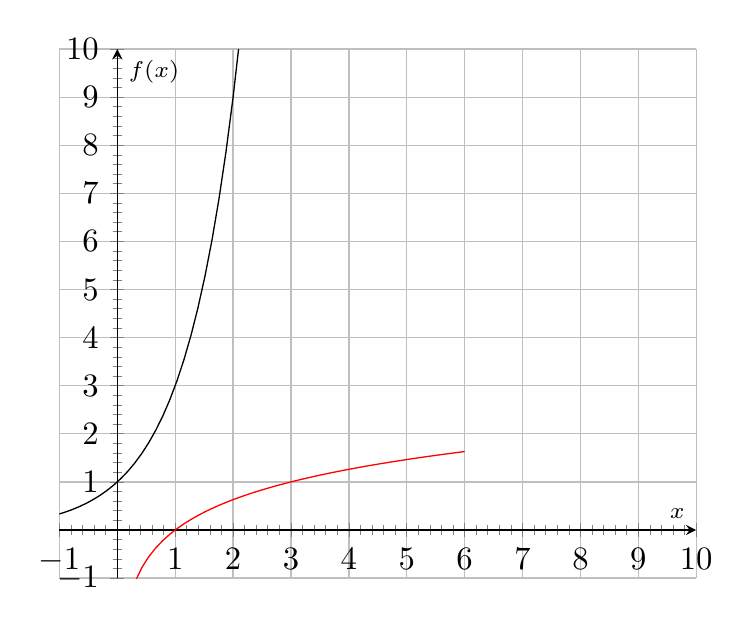
\begin{tikzpicture}[scale=1.18]
    \begin{axis}%
        [
            grid=major,
            xtick={-1,0,...,10},
            minor x tick num=4, % 4 minor ticks => 5 subintervals
            xmin=-1,
            xmax=10,
            xlabel={\scriptsize $x$},
            axis x line=middle,
            ytick={-1,0,...,10},
            minor y tick num=4,  % 4 minor ticks => 5 subintervals
            ymin=-1,
            ymax=10,
            ylabel={\scriptsize $f(x)$},
            axis y line=middle,
            no markers,
            samples=100,
            domain=-6:6
        ]
        \addplot[black] (x,{3^x});
        \addplot[red] (x,{ln(x)/ln(3)}); 
    \end{axis}
\end{tikzpicture}

\subsubsection{Graphen schneiden mit TR}

\hfill \break
Example:\\
\fboxrule=0.8pt \fcolorbox{black}{lightgray}{%
    \begin{tabular}[t]{@{}l@{}}
        $y = -x^3+8x-3$    \\
        $y = x^2-6x+9$     \\
        \\
        2nd calc intersect \\
        \\
        $S(1\vert4)$       \\
        $S(6\vert 9)$      \\
    \end{tabular}}\\
